\documentclass[11pt,a4paper]{article}
\usepackage[margin=2.1cm]{geometry}
\usepackage{booktabs}
\usepackage{tabularx}
\usepackage{longtable}
\usepackage{array}
\usepackage{graphicx}
\usepackage{pdflscape}
\usepackage{tikz}
\usepackage{tikz-timing}
\usetikzlibrary{positioning,arrows.meta}
\usepackage{xcolor}
\usepackage{enumitem}
\usepackage{listings}
\usepackage{caption}
\usepackage[hidelinks]{hyperref}
\usepackage{fancyhdr}

\definecolor{codebg}{HTML}{F4F7F6}
\definecolor{teal}{HTML}{0B7670}
\newcommand{\sig}[1]{\texttt{#1}}
\setlist{itemsep=2pt,topsep=4pt}
\setlength{\parskip}{4pt}
\setlength{\parindent}{0pt}
\lstset{basicstyle=\ttfamily\small,backgroundcolor=\color{codebg},frame=none,xleftmargin=6pt,xrightmargin=6pt,aboveskip=6pt,belowskip=6pt,columns=fullflexible,keepspaces=true,showstringspaces=false}
\tikzset{timing/d/text/.style={font=\scriptsize},timing/rowdist=2.6ex}

\pagestyle{fancy}
\fancyhf{}
\lhead{\small Paul Vincent Bezzina \textbar{} ProEm - Open Source Protocol Emulator}
\rhead{\small Design reference v1.1}
\cfoot{\small\thepage}

\title{ProEm: Protocol Emulator ASIC\\\large Design Reference}
\author{Paul Vincent Bezzina}
\date{17 October 2026}

\begin{document}
\maketitle
\thispagestyle{fancy}

\begin{center}
\begin{tabularx}{\linewidth}{@{}l>{\raggedright\arraybackslash}X@{}}
\toprule
Process & IHP SG13CMOS5L 130\,nm, through Tiny Tapeout (6 $\times$ 4 tiles) \\
System clock & 50\,MHz (10BASE-T transmit needs 40 or 60\,MHz) \\
Channels & 2 independent protocol channels, A and B \\
Host link & UART in (auto-baud), UART out (rate set by \sig{LINK}) \\
Standards verified & UART, SPI (controller in all four modes, and target), I\textsuperscript{2}C (controller and target), PS/2, 10BASE-T receive, Manchester transmit, USB low speed receive and transmit with CRC and handshake, SWD-style acknowledge handling, CAN with bit stuffing, arbitration, CRC-15 and acknowledge, and 16 more in the \emph{Standards Programming Guide} (RS-485 to RC5 infrared) \\
Logic & 18,969 cells after synthesis, 25,612 after place and route (43\,\% of the core) \\
Timing & met at all three corners after routing; 3.84\,ns setup slack at 1.08\,V, 125\,$^\circ$C (62\,MHz) \\
Instruction set & ISA v0.7.1 (separate document: \emph{ProEm Instruction Set}) \\
\bottomrule
\end{tabularx}
\end{center}

\tableofcontents
\newpage

\section{Overview}

ProEm is an open-source protocol emulator ASIC. The chip lets an RP2040 speak many serial protocols through one piece of hardware. The RP2040 does not bit-bang anything. It describes a frame to the chip in a few instruction bytes: how the frame starts, which fields follow, which way each field goes, how the frame ends, how the line is coded and where the bit clock comes from. The chip then runs the frame at up to one bit per system clock, with exact timing, and sends back what it received together with a status for every frame.

The design has four parts:
\begin{enumerate}
\item \textbf{Host side.} A UART receiver with auto-baud feeds the control unit, which decodes ISA v0.7.1 instructions into registered configuration writes. A return path sends received data, frame status and link events back on a second UART.
\item \textbf{Input pipeline.} Every input pin passes through two synchroniser flip-flops and one more register before any logic uses it.
\item \textbf{Two channels.} Each channel has a host FIFO for write data, a \emph{frame chain} that runs the frame, an \emph{entry dispatcher}, and a \emph{line codec} that turns pins into bits and ticks, and bits into pin levels.
\item \textbf{Outputs.} Each channel drives a data output, a pair output (the complement, for USB D$-$), a clock output and a select output, each with an output enable. Bidirectional pads are read back through the input pins.
\end{enumerate}

The two channels run at the same time. That is how the chip does SPI full duplex (one channel writes MOSI, the other reads MISO), UART receive and transmit together, or a transmitter looped into a receiver for self-test.

\begin{landscape}
\begin{figure}[p]
\centering
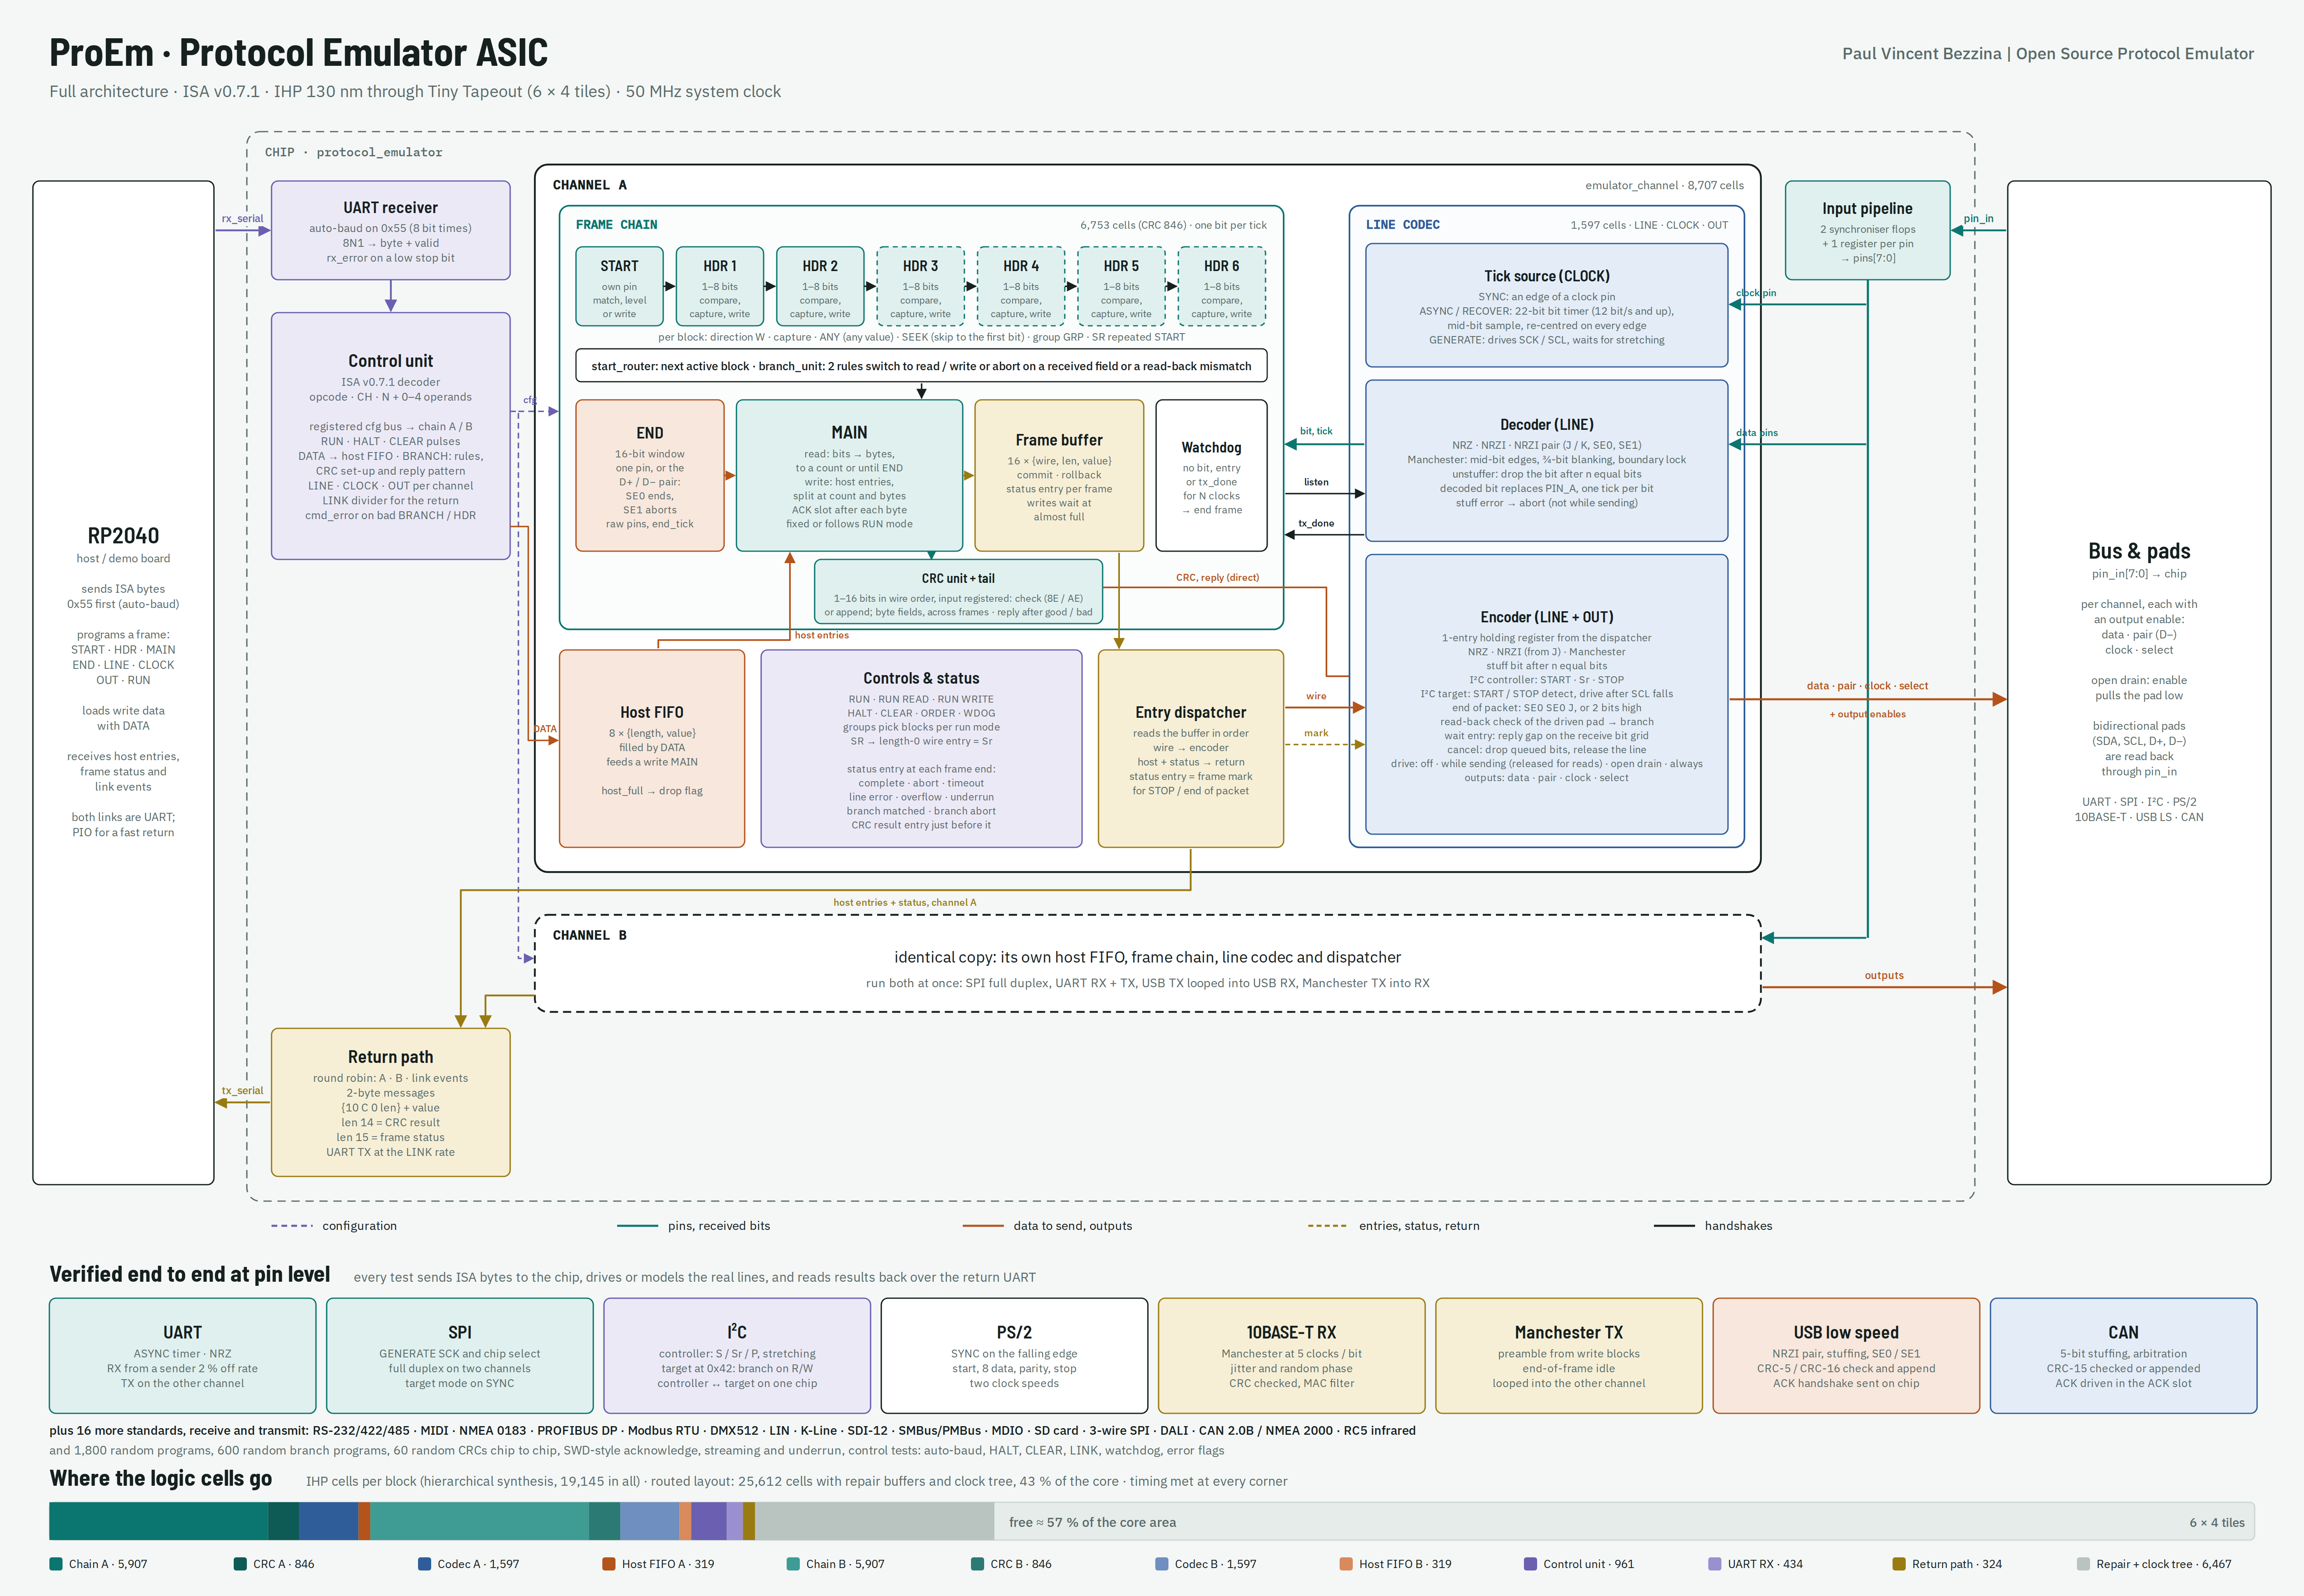
\includegraphics[width=\linewidth,height=0.9\textheight,keepaspectratio]{../images/protocol_emulator_architecture.png}
\caption{The whole chip. Channel A is shown in full; channel B is an identical copy.}
\label{fig:arch}
\end{figure}
\end{landscape}

\section{Top-level interface}

The top module is \sig{protocol\_emulator}. Its ports are generic; the Tiny Tapeout wrapper maps them onto \sig{ui\_in}, \sig{uo\_out} and the bidirectional \sig{uio} pins.

\begin{center}
\begin{tabularx}{\linewidth}{@{}l l >{\raggedright\arraybackslash}X@{}}
\toprule
Port & Dir & Meaning \\
\midrule
\sig{clk}, \sig{rst\_n} & in & System clock and active-low asynchronous reset \\
\sig{rx\_serial} & in & Instruction bytes from the RP2040, 8N1. The first byte after reset must be \texttt{0x55} \\
\sig{pin\_in[7:0]} & in & Protocol input pins, shared by both channels \\
\sig{tx\_serial} & out & Return UART to the RP2040 \\
\sig{data\_out\_x}, \sig{data\_oe\_x} & out & Channel x data output and output enable. In open-drain mode \sig{out} is 0 and \sig{oe} pulls the pad low \\
\sig{pair\_out\_x}, \sig{pair\_oe\_x} & out & Complement of the data output (USB D$-$) \\
\sig{clock\_out\_x}, \sig{clock\_oe\_x} & out & Generated clock (SCK, SCL) \\
\sig{select\_out\_x} & out & Chip select: active from the frame's START until its last bit has gone out \\
\sig{armed\_x}, \sig{host\_full\_x}, \sig{baud\_locked} & out & Debug status \\
\bottomrule
\end{tabularx}
\end{center}

\paragraph{Pads.} A bidirectional line such as SDA is a pad driven by \sig{data\_out}/\sig{data\_oe} and read back on one of the \sig{pin\_in} bits. I\textsuperscript{2}C uses open drain on both SDA and SCL, so the pads need external pull-ups. USB low speed needs 1.5\,k$\Omega$ from D$-$ to 3.3\,V when the chip is the device, and the pad voltage must reach 2.8\,V or a transceiver is needed.

\paragraph{Input latency.} The pipeline adds three clocks between a pad and the logic. Every pin is delayed equally, so a data pin and a clock pin stay aligned.

\section{Blocks}

\subsection{UART receiver and auto-baud (\sig{uart\_rx})}

After reset the receiver waits for the first falling edge, then counts clocks until the fifth falling edge. For \texttt{0x55} those five edges are exactly 8 bit times apart, so the clocks per bit are the count divided by 8. The receiver then waits for the stop bit and becomes a normal 8N1 receiver at that rate. The sync byte is not passed on. A byte whose stop bit is low raises \sig{rx\_error}. The measured rate is also the default rate of the return UART.

\subsection{Control unit (\sig{control\_unit})}

The control unit reads an opcode byte \texttt{\{OP, CH, N\}}, collects 0--4 operand bytes, and in one further clock turns the instruction into:
\begin{itemize}
\item a write on the shared configuration bus with a write enable for channel A or B (\sig{START}, \sig{HDR}, \sig{MAIN}, \sig{END}, \sig{WDOG}, \sig{ORDER});
\item a pulse: \sig{RUN} with its mode, \sig{HALT} or \sig{CLEAR};
\item a host FIFO write (\sig{DATA});
\item a register update: \sig{LINE}, \sig{CLOCK} and \sig{OUT} per channel, \sig{LINK} for the return link.
\end{itemize}
Every output is a register, so the configuration bus forms a pipeline stage and the decode logic is never in a channel's timing path. \sig{START} patterns are given as plain numbers; the control unit aligns them for the channel's bit order. \sig{BRANCH} rules travel on the same bus (select 8 and 9). \sig{BRANCH} with \sig{N} $>$ 4 and \sig{HDR 0}/\sig{HDR 7} raise \sig{cmd\_error}.

\subsection{Frame chain (\sig{frame\_chain})}

The frame chain is the frame engine: one START block, up to six header blocks and one MAIN block, run strictly in order, one bit per tick.

\begin{itemize}
\item \textbf{START} slides an 8-bit window over its own pin and matches a pattern of 1--8 bits; with 0 bits it waits for a level (SPI chip select); as a write block it sends its value when \sig{RUN} starts the frame.
\item \textbf{Headers} each compare, capture or send a 1--8 bit field. Each has a group (always, read runs, write runs) and an optional repeated START before it. A read header with \sig{ANY} accepts any value and keeps what arrived, in place of its compare value.
\item \textbf{start\_router} enables the next active block after the previous one succeeds. It skips unconfigured blocks and blocks whose group is not in the current run mode.
\item \textbf{branch\_unit} holds two \sig{BRANCH} rules. When a watched block succeeds, a rule compares its value under a mask and chooses an action: keep the mode, switch to read, switch to write, or abort. A second kind of rule fires when the codec reports that the line read back differently from what the chip drove. The decision is registered, and the chain pauses for that one clock so the next block starts in the new mode. A branch abort keeps the values captured so far and stops the codec driving at once.
\item \textbf{MAIN} reads bits into bytes, to a count or until END; or writes host entries, splitting them at the frame's bit count and, with the ACK slot on, at byte edges. After each byte it can add one bit the other way (I\textsuperscript{2}C ACK). Its direction is fixed or follows the run mode.
\item \textbf{END} slides a 16-bit window over one raw pin, or over the D+/D$-$ pair compare: both low (SE0) is a 1, both high (SE1) aborts with a line error. After an abort, START waits until END has matched again, so it never searches inside the rest of a rejected frame.
\item \textbf{crc\_unit} holds one CRC register of 1 to 16 bits, kept top aligned in 16 bits so every width uses the same shifter. It takes up to 8 bits per clock in wire order: single received bits as they are sampled (after unstuffing), the START value when it matches, and each written entry as it enters the frame buffer. The chain registers what it feeds, so the register takes the bits one clock after they are sampled or written. It is reloaded with its initial value whenever no frame is running. Its \sig{good} output compares the register with the residue; its \sig{crc\_out} output is the register, inverted if asked.
\item \textbf{Tail} runs after MAIN ends, before the frame completes, when the CRC or the reply is configured. Each step waits until the CRC register has taken every earlier bit, so the tail starts one clock after MAIN's last bit. It has up to six steps, each done once: the CRC result entry (read frames with check on), two CRC entries of up to 8 bits (write frames with append on), the reply gap, and two reply entries. The result goes into the frame buffer as a host entry; the CRC, gap and reply entries go straight to the codec once every earlier wire entry of the frame has been handed over, so they are never queued behind received data waiting for the return link. The reply is decided at the gap step, after the last received bit has reached the CRC. A rule with \sig{SRC} = 1, \sig{BLOCK} = 1 fires when the result entry is pushed.
\item \textbf{Watchdog} ends a frame when no bit, host entry or sent entry is seen for a set number of clocks.
\item \textbf{Frame buffer} holds 16 entries \texttt{\{wire, length, value\}}. Written values are released at once; captured values are released when MAIN starts and dropped on abort. At the end of every frame the chain adds a \emph{status entry} (length 15) with complete, abort, timeout, line error, overflow, underrun, branch-matched and branch-abort flags.
\end{itemize}

Read blocks only take ticks once every bit written ahead of them has left the chip (\sig{line\_free}), so a frame can send a request and then read the reply. Write blocks wait when the buffer is almost full, so written bits are never lost; received entries that arrive with the buffer full are dropped and the frame's status has the overflow flag.

\paragraph{Streaming and underrun.} A write MAIN takes host entries as they arrive, so \sig{DATA} can keep coming during the frame. With a generated clock the line simply pauses when the host FIFO is empty. On a line with fixed timing (ASYNC, RECOVER, SYNC) the chain aborts with the \emph{underrun} flag when MAIN needs data, none is waiting and every queued bit has gone out, and the codec stops driving. While a read-back \sig{BRANCH} rule is set, a write frame also stays open until its last bit has left the pin, so an arbitration loss in the last bits still reaches the frame's status.

\subsection{Host FIFO and entry dispatcher}

The host FIFO holds 8 \texttt{\{length, value\}} entries loaded by \sig{DATA} and feeds a write MAIN. A \sig{DATA} arriving while it is full is dropped and reported as a link event.

The entry dispatcher reads the frame buffer in order. Wire entries go to the codec's encoder; host entries and status entries go to the return path. After a cancel (branch abort, underrun, I\textsuperscript{2}C bus error) it discards the frame's remaining wire entries up to its status entry, and the chain's count of bits in flight is kept consistent. When a status entry reaches the head, every bit of that frame has already been handed to the encoder, so the dispatcher gives the encoder a \emph{frame mark} at that moment. The encoder uses it to send the I\textsuperscript{2}C STOP or the end of packet at exactly the right place.

\subsection{Line codec (\sig{line\_codec})}

The codec sits between the pins and the frame chain. \sig{CLOCK} chooses the tick source, \sig{LINE} the line code, \sig{OUT} the output behaviour. The separate \emph{Line Codec} reference (\sig{docs/line\_codec.pdf}) explains it signal by signal.

\paragraph{Tick source.}
\begin{itemize}
\item \textbf{SYNC}: a tick on the rising, falling or both edges of a clock pin (SPI target, PS/2, a read-back clock).
\item \textbf{ASYNC / RECOVER}: a bit timer of \sig{DIV} clocks per bit that samples mid-bit and re-centres on every edge of the data line. The decoded bit replaces \sig{LINE}'s \sig{PIN\_A} in the pins the chain sees, with one tick per bit.
\item \textbf{GENERATE}: the codec drives the clock output, \sig{DIV} clocks per half period, only while a bit is waiting to go out or a read block wants one. The sampling edge gives the tick. With open drain it waits for the clock read-back pin to go high, which gives I\textsuperscript{2}C clock stretching.
\end{itemize}

\paragraph{Decoder.} NRZ takes the mid-bit sample. NRZI compares it with the previous one (same = 1). The NRZI pair code reads J/K from D+ and D$-$ and gives no bits during SE0 or SE1. Manchester decodes on the mid-bit edges: the new level is the bit, and edges within $\frac34$ of a bit after an accepted edge are ignored, which skips the boundary edges between equal bits. An unstuffer drops the bit after $n$ equal bits; a stuffed bit with the wrong value aborts the frame with a line error.

\paragraph{Encoder.} It holds one entry from the dispatcher and sends it bit 0 first (the chain has already reversed MSB-first fields). It encodes NRZ, NRZI starting from J, or Manchester, inserts a stuff bit after $n$ equal bits, and continues seamlessly into the next entry. In I\textsuperscript{2}C mode it sends START before a transaction, repeated START for a length-0 entry, and STOP at the frame mark. With end of packet on, the frame mark produces two bit times of SE0 and one of J on a pair, or two bit times high on a single line. \sig{tx\_done} after each entry lets the chain know the line is free.

\begin{figure}[h]
\centering
\begin{tikztimingtable}[timing/slope=0.12,xscale=1.9,yscale=1.1]
UART \texttt{0x48} & 2H 4L H 2L H L 2H \\
 & 2D{idle} D{S} D{0} D{0} D{0} D{1} D{0} D{0} D{1} D{0} 2D{stop} \\
\extracode
\end{tikztimingtable}

\vspace{8pt}
\begin{tikztimingtable}[timing/slope=0.12,xscale=1.9,yscale=1.1]
USB D+ & L 7H 5L \\
USB D$-$ & H 7L 2H 2L H \\
 & D{J} D{0} 6D{six 1s: no change} D{st} D{1} 2D{SE0} D{J} \\
\end{tikztimingtable}

\vspace{8pt}
\begin{tikztimingtable}[timing/slope=0.12,xscale=1.9,yscale=1.1]
Manchester & L 2H 2L H L 2H L \\
 & 2D{1} 2D{0} 2D{1} 2D{1} 2D{0} \\
\end{tikztimingtable}
\caption{Three line codes from the same codec. UART: NRZ, LSB first, start and stop bits. USB low speed: NRZI on D+/D$-$ (a 0 changes the line), a stuff bit (st) after six 1s, then the end of packet. 10BASE-T: Manchester, low-to-high in the middle of the bit = 1.}
\end{figure}

\paragraph{I\textsuperscript{2}C target.} With \sig{OUT I2C} and a SYNC clock on SCL, the codec detects START and STOP (SDA falling or rising while SCL is high), which start the frame and end a MAIN that waits for END. A bit to send waits for SCL to fall before it is driven, and SDA is released after the falling edge that ends it, so the address ACK and data bytes meet the I\textsuperscript{2}C set-up and hold rules. The chip never drives SCL in this mode.

\paragraph{Read-back check and cancel.} While sending, the codec compares the pad it drives (read back on \sig{LINE}'s \sig{PIN\_A}) with the level it wants, in the middle of each bit. A difference is passed to the branch unit (CAN-style arbitration). On a cancel the encoder drops its current and next entry, releases the line and counts the dropped entries as sent.

\paragraph{Outputs.} \sig{DRIVE} is off after reset, push-pull while sending, open drain, or push-pull always (with an idle level, for a UART line). The pair output carries the complement. The select output is active from the frame's START until its last bit has gone out.

\subsection{Return path (\sig{return\_path}, \sig{uart\_tx})}

The return path takes host entries and status entries from both channels and link events, in round robin, and sends each as a two-byte message on the return UART at the \sig{LINK} rate (or the auto-baud rate when \sig{LINK} is 0).

\section{Host protocol}

\subsection{Start-up}

\begin{enumerate}
\item Release reset and hold \sig{rx\_serial} high for at least one byte time.
\item Send \texttt{0x55}. The chip measures the rate from it; \sig{baud\_locked} goes high.
\item Optionally send \sig{LINK} to speed up the return link (\texttt{E0 00 04} = 4 clocks per bit, 12.5\,Mbaud at 50\,MHz).
\item Program each channel: \sig{LINE}, \sig{CLOCK}, \sig{OUT}, \sig{ORDER}, \sig{WDOG}, the blocks, then \sig{RUN}.
\end{enumerate}

\sig{CLEAR} returns a channel to its reset state, including its outputs; \sig{HALT} stops a frame and disarms the channel but keeps its program.

\subsection{Return messages}

\begin{center}
\begin{tabularx}{\linewidth}{@{}l l >{\raggedright\arraybackslash}X@{}}
\toprule
First byte & Second & Meaning \\
\midrule
\texttt{10 C 0 LLLL} & value & Host entry from channel \texttt{C}, length 0--8. Length 0 with value \texttt{02} is a NACK from a writing MAIN \\
\texttt{10 C 0 1110} & result & CRC result of a read frame: bit 0 good, bit 1 checked. Comes after the frame's data and before its status \\
\texttt{10 C 0 1111} & flags & End of a frame on channel \texttt{C}: bit 0 complete, 1 abort, 2 timeout, 3 line error, 4 overflow, 5 underrun, 6 branch matched, 7 branch abort \\
\texttt{11 000000} & flags & Link events: bit 0 \sig{rx\_error}, 1 \sig{cmd\_error}, 2 \sig{DATA} dropped on A, 3 on B \\
\bottomrule
\end{tabularx}
\end{center}

A frame's host entries always come before its status message. A simple receiver on the RP2040:

\begin{lstlisting}[language=C]
void on_return_message(uint8_t head, uint8_t value) {
    if ((head & 0xC0) == 0xC0) { link_events(value); return; }
    int chan = (head >> 5) & 1, len = head & 0x0F;
    if (len == 15) frame_done(chan, value);        /* status flags   */
    else if (len == 14) crc_result(chan, value);   /* bit 0 good     */
    else           frame_data(chan, len, value);   /* 0..8 bits      */
}
\end{lstlisting}

\subsection{Choosing \sig{RUN} modes}

\begin{itemize}
\item \textbf{Receiving:} plain \sig{RUN} arms the channel; it stays armed after every frame.
\item \textbf{Packets} (USB, Ethernet, I\textsuperscript{2}C transactions): load the data with \sig{DATA}, then \sig{RUN WRITE} or \sig{RUN READ}. The channel starts exactly one frame per \sig{RUN}.
\item \textbf{Streams} (UART transmit): plain \sig{RUN}. The channel also starts a new frame whenever data is waiting.
\item \textbf{Long packets}: load a few \sig{DATA} entries, send \sig{RUN WRITE}, then keep sending \sig{DATA} while the frame runs. Watch \sig{HOST\_FULL}; on a fixed-timing line keep ahead of the line or the frame ends with an underrun (status \texttt{22}).
\item \textbf{Reacting to the other side} (I\textsuperscript{2}C target, SWD, arbitration): add \sig{BRANCH} rules; the status byte's bits 6 and 7 say which way the frame went.
\end{itemize}

\section{Protocol recipes}

Each recipe lists the instruction bytes. The bytes were produced by the test bench's own encoder, and the same programs (with smaller dividers, to keep simulation short) pass the tests in Section~\ref{sec:verify}. Dividers are for a 50\,MHz clock.


\paragraph{UART receive, 115\,200 baud, channel A.} RX on pin 0. \sig{LINE} none on pin 0; \sig{CLOCK} ASYNC, 434 clocks per bit; START reads the start bit; MAIN reads 8 data bits and the stop bit.
\begin{lstlisting}
A0 00 00   B0 40 00 01 B2   10 01 00 00   30 00 00 09   70
\end{lstlisting}


\paragraph{UART transmit, channel B.} Push-pull output, idle high; START writes the start bit; MAIN writes 9 bits. Each byte is two \sig{DATA} entries: the byte and a stop bit.
\begin{lstlisting}
A8 00 00   B8 40 00 01 B2   D8 E0   18 81 00 00   38 40 00 09
CF 48   C8 01   78                                  ("H", then RUN)
\end{lstlisting}


\paragraph{SPI controller, mode 0, MSB first, full duplex.} Channel A generates SCK (half period 6 clocks) and chip select, writes MOSI from \sig{DATA}. Channel B reads MISO on pin 3, clocked by SCK read back on pin 1, started by chip select read back on pin 2.
\begin{lstlisting}
A: 61   A0 00 00   B0 81 00 00 06   D0 C0   50 0F A0   10 80 00 00   30 40 00 10
B: 69   A8 03 00   B8 01 00 00 00   18 00 02 00   38 03 00 10   78
transfer:   C7 A5   C7 5A   70
\end{lstlisting}


\paragraph{I\textsuperscript{2}C controller, 100\,kHz, register read and write in one program.} Device 0x48, register 0x05. SDA read back on pin 0, SCL on pin 1; open drain with I\textsuperscript{2}C conditions.
\begin{lstlisting}
61   A0 00 00   B0 89 00 00 FA   D0 A4   50 EA 60
10 88 00 90   21 01 00 00   22 88 00 05   23 01 00 00
24 98 80 91   25 11 00 00   30 90 00 10
write:  C7 A1   C7 B2   72        bus: S 90 A 05 A A1 A B2 A P
read:   71                        bus: S 90 A 05 A Sr 91 A d0 A d1 N P
\end{lstlisting}


\paragraph{PS/2 keyboard to host, channel B.} Clock on pin 4 (falling edge), data on pin 5. Each key gives \texttt{\{8, code\}} and \texttt{\{2, parity + stop\}}.
\begin{lstlisting}
A8 05 00   B8 14 00 00 00   18 01 05 00   38 05 00 0A   78
\end{lstlisting}


\paragraph{10BASE-T receive, broadcast frames.} Manchester line on pin 0; END sees the line high for 8 clocks at the end of the frame; return link at 4 clocks per bit.
\begin{lstlisting}
E0 00 04   A0 60 00   B0 C0 40 00 05   10 08 00 D5
21 48 00 FF   22 48 00 FF   23 48 00 FF   24 48 00 FF   25 48 00 FF   26 48 00 FF
30 20 00 00   40 40 00 00 FF   70
\end{lstlisting}


\paragraph{Manchester transmit (6 clocks per bit, a 60\,MHz clock for 10\,Mb/s).} The preamble comes from START and six write headers; MAIN sends up to 8 \sig{DATA} bytes (SFD first); end of packet holds the line high for two bit times.
\begin{lstlisting}
A0 60 00   B0 C0 00 00 06   D0 48   10 88 00 55
21 88 00 55   22 88 00 55   23 88 00 55   24 88 00 55   25 88 00 55   26 88 00 55
30 40 00 40      then DATA entries and RUN WRITE (72)
\end{lstlisting}


\paragraph{USB low speed receive.} D+ on pin 0, D$-$ on pin 1; NRZI pair with unstuffing; END on the pair, 2 bit times of SE0, SE1 aborts.
\begin{lstlisting}
E0 00 04   A0 40 31   B0 C0 80 00 21   10 08 00 80   30 20 00 00
40 10 A1 00 03   70
\end{lstlisting}


\paragraph{USB low speed transmit, channel B.} SYNC from START, PID \texttt{0x4B} from a header, 32 data bits from \sig{DATA}, stuffing and end of packet.
\begin{lstlisting}
A8 40 31   B8 C0 00 00 21   D8 58   18 88 00 80   29 88 00 4B   38 40 00 20
CF FF   CF FF   CF 7E   CF 00   7A
\end{lstlisting}


\paragraph{I\textsuperscript{2}C target at address 0x42.} SDA on pin 0, SCL on pin 1. The R/W bit is captured with \sig{ANY}; the branch makes MAIN write (the controller reads) or read (the controller writes); MAIN ends at STOP or repeated START.
\begin{lstlisting}
61   A0 00 00   B0 01 00 00 00   D0 84   10 00 00 00   21 07 00 42
22 41 40 00   23 81 00 00   F0 92 01 01   30 B0 00 40   70
data for reads:   C7 5A   C7 C3
\end{lstlisting}


\paragraph{SWD-style read with acknowledge check.} SWCLK generated (1\,MHz), SWDIO open drain on pin 0, LSB first. Only an OK acknowledge continues to the 33-bit data phase; WAIT and FAULT abort with the acknowledge returned.
\begin{lstlisting}
60   A0 00 00   B0 81 00 00 19   D0 80   10 88 00 A5
21 01 40 00   22 43 40 00   F0 72 07 01   30 00 00 21   70 (each transaction)
\end{lstlisting}


\paragraph{CAN-style arbitration.} 1\,Mbit/s (50 clocks per bit), open drain, read back on pin 0. A lost arbitration aborts the frame and releases the line in the same bit (status \texttt{C2}).
\begin{lstlisting}
61   A0 00 00   B0 40 00 00 32   D0 80   10 81 00 00   30 40 00 13   F0 C8 00 00
C7 id[10:3]   C2 id[2:0]   C7 data   72
\end{lstlisting}


\section{Verification}\label{sec:verify}

The test bench (\sig{sim/bench.h}) simulates the whole chip with Yosys CXXRTL. Every test does what the RP2040 would do: it resets the chip, sends \texttt{0x55}, sends instruction bytes on \sig{rx\_serial}, and decodes the return UART on \sig{tx\_serial} into host entries, frame status and link events. Protocol lines are driven or modelled at the pins every clock: open-drain buses are wired-AND, clocks are looped back through \sig{pin\_in}, and devices are behavioural models.

\begin{longtable}{@{}>{\raggedright\arraybackslash}p{2.6cm} >{\raggedright\arraybackslash}p{12.2cm} l@{}}
\toprule
Test & What it checks & Result \\
\midrule
\endhead
\sig{t\_control} & Auto-baud at 16 and 7 clocks per bit; read frames; header mismatch; watchdog timeout; \sig{HALT}, re-\sig{RUN}; \sig{CLEAR}; START alignment in both bit orders; \sig{LINK}; \sig{cmd\_error}, \sig{rx\_error}; \sig{DATA} dropped on a full FIFO & Pass \\
\sig{t\_uart} & Channel A receives 5 bytes from a sender 2\,\% fast, then 2\,\% slow; channel B transmits ``Hi!'' decoded by a model & Pass \\
\sig{t\_spi} & Controller full duplex against a slave model; target mode against a master model; SCK half period 4, 6, 12 clocks & Pass \\
\sig{t\_i2c} & Device model on an open-drain bus: \sig{RUN WRITE}, \sig{RUN READ} with Sr, clock stretching, address NACK with STOP; SCL half period 4, 10, 25 & Pass \\
\sig{t\_ps2} & Four keys with parity and stop bits at two clock rates & Pass \\
\sig{t\_ethernet} & Manchester line timed in nanoseconds with $\pm$3\,ns jitter and random phase at 50 and 60\,MHz; all broadcast frames intact and CRC checked, other addresses rejected; a 64-byte frame reported as overflow & Pass \\
\sig{t\_manchester} & Manchester transmit at 6 and 10 clocks per bit, decoded by the other channel; end-of-frame idle and release & Pass \\
\sig{t\_usb} & Receive with stuffing at 33.33 clocks per bit; SE1 and missing stuff bit abort with line error; transmit decoded by a model, end of packet SE0 SE0 J then released; channel B transmit looped into channel A receive & Pass \\
\sig{t\_random} & 1,800 random programs (6 seeds $\times$ 150, both bit orders): 0--6 headers, fields of 1--8 bits, capture on and off, random data, mismatches, splits across frames & Pass \\
\sig{t\_i2c\_target} & Chip as I\textsuperscript{2}C target at 0x42 against a controller model: write of two bytes, read of two bytes (branch to write, controller NACK), wrong address (no ACK, abort), register write then repeated START and read; SCL at 417\,kHz and 1\,MHz & Pass \\
\sig{t\_branch} & SWD-style acknowledge: OK continues to 33 data bits, WAIT and FAULT abort with the acknowledge returned. CAN-style arbitration on an open-drain line against a node model: the chip wins, the chip loses and releases the line within the bit, and the channel is reusable afterwards & Pass \\
\sig{t\_stream} & Underrun: 8 of 32 bits loaded on a UART line aborts with status \texttt{22}. UART stream of 12 bytes (36 entries) fed while the frame runs. SPI stream of 20 bytes with the generated clock pausing & Pass \\
\sig{t\_standards} & Sixteen further standards, receive and transmit, each against a model of the other side (42 checks): RS-232/422/485 (driver enable on the select output), MIDI, NMEA 0183, PROFIBUS DP, Modbus RTU (CRC checked on chip with \sig{BYTE} and \sig{SPAN}), DMX512 (break detection by a framing abort), LIN master and slave (seeking header across a gap), K-Line fast and 5-baud init, SDI-12, SMBus with PEC (checked on chip), MDIO (PHY switching 0\,ns after MDC, push-pull), SD card CMD0 and CMD8 with the CRC-7 from the chip, 3-wire SPI (push-pull, no overlap), DALI (Manchester decoder with boundary lock), CAN 2.0B extended frames (NMEA 2000) and RC5 infrared (1.778\,ms bits, 22-bit divider). The programs are listed in the \emph{Standards Programming Guide} & Pass \\
\sig{t\_crc} & USB DATA0 receive with CRC-16: good packet answered with an ACK handshake 3 bit times after the end of packet, corrupted packet gets no reply, next packet good again; USB token CRC-5 good and bad; USB DATA1 transmit with CRC-16 appended and inverted, decoded by a model; CAN frame with bit stuffing from a node model, CRC-15 good (dominant ACK in the ACK slot), corrupted (no ACK), and a heavily stuffed ID; CAN chip to chip on a wired-AND bus, B appends the CRC and A checks it and acknowledges; 60 random CRCs (width 1--16, random polynomial, init, inversion, bit order and length, a third corrupted on the wire) looped from B to A & Pass \\
\sig{t\_random\_\allowbreak branch} & 600 random branch programs (3 seeds $\times$ 100, both bit orders): a capture-any header of 1--8 bits, random mask and value (half forced to match), random hit and miss actions, random base run mode, read-group and write-group headers; checks the path taken, the captures and the status byte & Pass \\
\sig{t\_modes} & SPI controller in all four modes at 3 and 6 clocks per half period, writing into a device model that samples with no hold margin and reading its reply; both \sig{BRANCH} rules aborting on their own value; \sig{NOP} accepted without an error & Pass \\
\bottomrule
\end{longtable}

\paragraph{Tiny Tapeout test.} \sig{test/test.py} (cocotb, Icarus Verilog) drives the Tiny Tapeout top level through its pads: auto-baud and the \sig{cmd\_error} event; a UART loopback from channel B's data pad into channel A; an SPI loopback in which channel A generates SCK and MOSI on its pads and channel B samples them back, gated by channel A's chip select; an I\textsuperscript{2}C loopback in which channel A is the controller and channel B the target at 0x42 on the same open-drain wire; sending ``A0000'' over UART with the host library; and a CRC-8 loopback, channel B appending the CRC and channel A checking it, with the right residue (result \texttt{03}) and a wrong one (\texttt{02}). It passes on the RTL and is run on the gate-level netlist by the \sig{gds} workflow.

\paragraph{Bugs found by these tests and fixed.}
\begin{itemize}
\item The frame buffer's full check compared a 32-bit difference; after the pointers wrapped it never saw ``full'' and overwrote unread entries.
\item Header and START pushes are registered, so write backpressure must stop at ``almost full''.
\item Chip select glitched between a write frame completing and its last bits reaching the codec.
\item STOP and the end of packet waited for the return link; they now follow the frame mark.
\item Outputs drove low after reset; they are now off until \sig{OUT} is given.
\item A write frame finishes as soon as its last bits are queued, before they leave the pin, so a read-back rule had no frame left to act on (found by the CAN-style test). Write frames now stay open until the line drains while such a rule is set.
\item The CAN start-of-frame bit was dropped as a stuff bit when it followed five or more idle recessive bits; unstuffing now counts only inside a frame (found by the CAN CRC test).
\item A transmit with the chain's own data pin not read back raised a stuff error and aborted the frame; stuff errors are now ignored while the chain itself is driving the line.
\item The reply was queued in the frame buffer behind received data and reached the line about 10 bits late on CAN; the tail now hands its wire entries straight to the codec.
\item Timing: the first branch design fed the new mode straight into MAIN in the same clock, adding about 5\,ns to the worst path. The decision is now registered and the chain pauses for one clock.
\item A second cancel within two clocks of the first, or an entry finishing on the same clock as a pending drop, lost one \sig{tx\_done}; the channel then never listened again until \sig{CLEAR} (found by the line codec proof, v0.7.1).
\item In SPI modes 1 and 3 the generated-clock path changed the data pin on the device's sampling edge, leaving no hold time; the data is now held through that edge (found through a coverage gap, v0.7.1).
\end{itemize}

\paragraph{Further checks.} The verification report (\sig{docs/verification\_report.pdf}) records the full sign-off of v0.7.1, and the toolchain guide explains how to run each check.
\begin{itemize}
\item \textbf{Formal proofs.} Six modules are proven with SymbiYosys for every input sequence and with no depth limit (ABC \sig{pdr}); each harness in \sig{formal/} wraps the unchanged RTL with a small reference model. The host FIFO and the frame buffer: occupancy and flags exact, data out unchanged and in order, rollback discarding exactly the uncommitted entries. The UART transmitter: every frame exact for every ratio from 1 to 15. The branch unit: the two rules behave as the ISA describes. The CRC unit: the 8-bit-per-clock update equals a bit-by-bit reference CRC for every width, polynomial and chunk length. The line codec: every accepted entry is answered with exactly one \sig{tx\_done}, whatever the cancels, and the output enables obey \sig{DRIVE}.
\item \textbf{Lint.} Verilator with every warning on (\sig{scripts/lint.sh}) is clean; 13 reviewed waivers are recorded in \sig{lint/waivers.vlt}. There are no combinational loops (Yosys \sig{check -assert}).
\item \textbf{Second simulator and coverage.} Every pin-level test also runs on a Verilator model, which reports 98.7\,\% line and branch coverage over the whole regression (\sig{scripts/coverage.sh}).
\item \textbf{Independent decode.} The waveforms of the standards tests are decoded by sigrok's protocol decoders and checked against independently computed bytes: 30 of 30 pass (\sig{scripts/\allowbreak sigrok\_check.py}).
\item \textbf{Gate level.} The cocotb tests pass on the synthesised and on the routed netlist with the IHP cell models.
\end{itemize}

\section{Implementation results}

\subsection{Synthesis}

Yosys and ABC mapped to the IHP \sig{sg13cmos5l} cells, each block synthesised on its own:

\begin{center}
\begin{tabular}{@{}lr@{}}
\toprule
Block & Cells \\
\midrule
Frame chain & 5,907 \\
\quad of which CRC unit & 846 \\
Line codec & 1,597 \\
Host FIFO (8 entries) & 319 \\
One channel (chain, codec, host FIFO, dispatcher) & 8,707 \\
Control unit & 961 \\
UART receiver with auto-baud & 434 \\
Return path with UART transmitter & 324 \\
\midrule
\textbf{Whole design (two channels)} & \textbf{19,145} \\
\bottomrule
\end{tabular}
\end{center}

Flattened, as \sig{scripts/synth\_ihp.sh} does it, the design is 19,721 cells and 333,138\,$\mu$m$^2$, 36\,\% of the 6 $\times$ 4 tile area before the flow adds buffers and the clock tree.

\subsection{Place and route on Tiny Tapeout}

The design was hardened on the Tiny Tapeout CMOS5L template (the \sig{cmos5l} branch of the IHP template) with the flow its \sig{gds} workflow runs: LibreLane 3.1.0.dev3 and the IHP SG13CMOS5L PDK at the commit the workflow installs, at the 6 $\times$ 4 tiles the Jane Street challenge sets. Timing is from the routed design with extracted parasitics.

\begin{center}
\begin{tabular}{@{}ll@{}}
\toprule
Tiles & 6 $\times$ 4, 1289.28 $\times$ 710.64\,$\mu$m \\
Cells & 18,969 after synthesis; 25,612 after place and route, not counting fill \\
 & (2,763 flip-flops, 6,104 timing repair buffers, 362 clock tree cells) \\
Utilisation & 43\,\% of the core area \\
Routing & 0 violations after detailed routing, 0 antenna violations (51 diodes) \\
Sign-off & Magic DRC 0 errors; LVS clean \\
Wire length & 1.15\,m \\
\bottomrule
\end{tabular}
\end{center}

\begin{center}
\begin{tabular}{@{}lllll@{}}
\toprule
Corner & Setup slack at 50\,MHz & Hold slack & Maximum clock & Power \\
\midrule
Typical, 1.2\,V, 25\,$^\circ$C & 9.82\,ns & 0.29\,ns & 98\,MHz & 10.2\,mW \\
Slow, 1.08\,V, 125\,$^\circ$C & 3.84\,ns & 0.61\,ns & 62\,MHz & 8.1\,mW \\
Fast, 1.32\,V, $-40\,^\circ$C & 12.35\,ns & 0.10\,ns & 131\,MHz & 12.7\,mW \\
\bottomrule
\end{tabular}
\end{center}

The CMOS5L flow only enforces timing at the typical corner, so \sig{src/config.json} adds three settings to make the slow corner pass as well: a 0.75\,ns limit on signal transitions, 3\,ns resizer setup margins, and a second setup repair after global routing. The first layout of v0.7.1 still missed the slow corner by 3.8\,ns, on paths ending in the CRC register and the frame buffer. Four RTL changes closed it without changing what the pins do, apart from the CRC and reply starting one clock later: the CRC input is registered; MAIN keeps the bits left in a register; the host FIFO head and the frame buffer's fill level are registered, and the buffer writes its memory one clock later with a bypass; and the CRC update picks its length once, after all 8 steps. The verification report gives the slack after each step. Most of the power is the clock reaching the 2,763 flip-flops.

\begin{center}
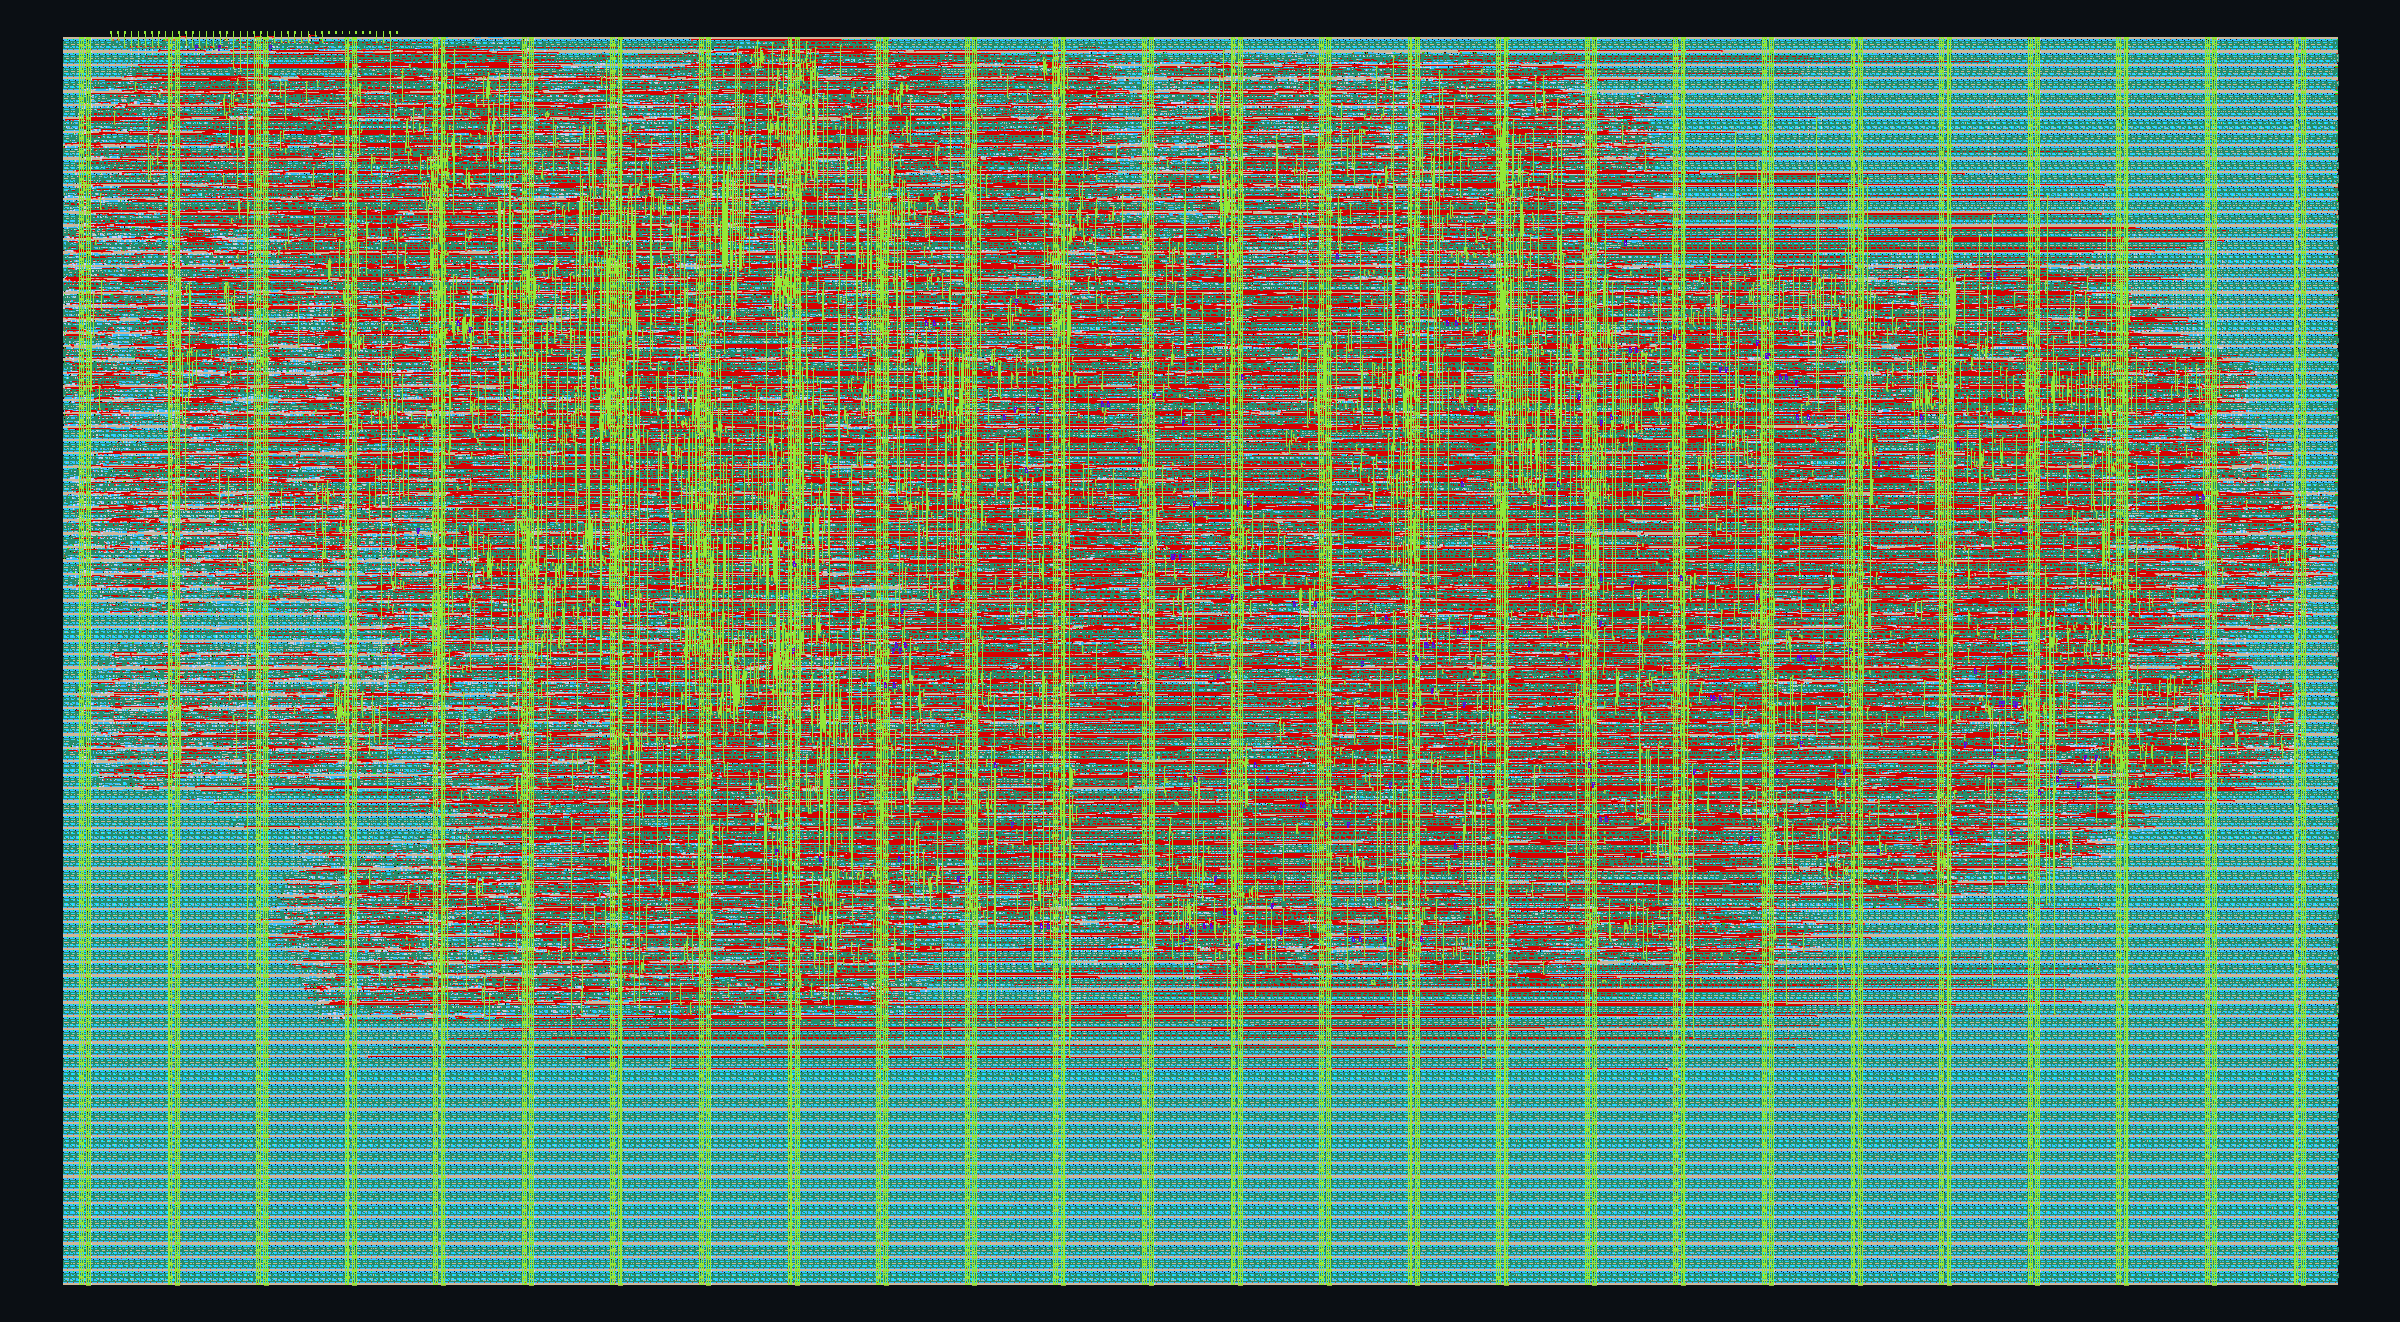
\includegraphics[width=\linewidth]{../images/layout_full.png}\\[2pt]
{\small Routed layout, 6 $\times$ 4 tiles. Cells cover 43\,\% of the core; the rest is filler and decoupling cells.}
\end{center}

\subsection{Pin map}

\begin{center}
\begin{tabularx}{\linewidth}{@{}llX@{}}
\toprule
Pin & Direction & Use \\
\midrule
\sig{ui[0]} & in & RX: instructions from the host (first byte \sig{0x55}) \\
\sig{uo[0]} & out & TX: data and status to the host \\
\sig{uo[1]} & out & BAUD\_LOCKED \\
\sig{uo[2]}, \sig{uo[3]} & out & ARMED for channels A and B \\
\sig{uo[4]}, \sig{uo[5]} & out & HOST\_FULL for channels A and B \\
\sig{uo[6]}, \sig{uo[7]} & out & SELECT (chip select) for channels A and B \\
\sig{uio[0]}--\sig{uio[2]} & in/out & pins 0--2, driven by channel A: data, pair, clock \\
\sig{uio[3]}--\sig{uio[5]} & in/out & pins 3--5, driven by channel B: data, pair, clock \\
\sig{uio[6]}, \sig{uio[7]} & in & pins 6 and 7 \\
\sig{ui[7:1]} & in & unused \\
\bottomrule
\end{tabularx}
\end{center}

The \sig{PIN} fields count the \sig{uio} pads. Every pad is read back through \sig{pin\_in}, so open-drain I\textsuperscript{2}C and the USB pair work on single pads; a channel drives its pads only when \sig{OUT} enables them.

\section{Limits and future work}

\begin{enumerate}
\item \textbf{Return link bandwidth.} Two bytes per host entry. At 4 clocks per bit the link keeps up with USB low speed and the clocked standards. Full-size 10BASE-T frames (64 bytes and more) arrive faster; they are received but overflow the 16-entry buffer and are reported with the overflow flag.
\item \textbf{Feeding fixed-timing lines.} \sig{DATA} streams during a frame, so packet length is no longer limited by the 8-entry host FIFO, but each entry costs 140 clocks on the instruction link at 7 clocks per bit. UART transmit keeps up to about 1.2\,Mbaud; faster fixed-timing lines must be preloaded (8 entries) or end with an underrun.
\item \textbf{Head-of-line blocking.} A host entry waiting for the return link holds up the wire entries behind it. I\textsuperscript{2}C just stretches SCL; a timed transmit would pause. The appended CRC and the reply are exempt.
\item \textbf{Manchester limits.} Receive needs at least 5 clocks per bit (50\,MHz for 10BASE-T); transmit needs an even divider (40 or 60\,MHz). The routed design's slowest path, 16.2\,ns at the slow corner, also fits a 60\,MHz clock (16.7\,ns), but the flow was only run at 50\,MHz.
\item \textbf{Not supported yet.} Clock stretching as an I\textsuperscript{2}C target; a \emph{loop} action for \sig{BRANCH} (repeat a block without the host); a CRC over Manchester lines with a reply gap (the gap needs a non-Manchester timed line).
\item \textbf{I\textsuperscript{2}C target speed.} Tested up to 1\,MHz SCL. Faster, the ACK after a repeated START can be late, because the previous frame's status entry must first reach the return link (head-of-line blocking).
\item \textbf{Reset.} \sig{CLEAR} resets a channel through its asynchronous reset (\sig{rst\_n \&\& !clear}), driven from a control-unit flip-flop.
\end{enumerate}

\section{Files}

\begin{center}
\begin{tabularx}{\linewidth}{@{}l>{\raggedright\arraybackslash}X@{}}
\toprule
Folder or file & Content \\
\midrule
\sig{info.yaml} & Tiny Tapeout project file: title, tile count, source list, pin names \\
\sig{src/top/} & \sig{tt\_um\_vertrex\_star\_proem.sv} (Tiny Tapeout top level and pin map), \sig{protocol\_emulator.sv} (chip core) and \sig{protocol\_emulator\_inst.sv} (instantiation template) \\
\sig{src/core/} & \sig{emulator\_channel}, \sig{control\_unit}, \sig{line\_codec}, \sig{entry\_dispatch}, \sig{return\_path} \\
\sig{src/core/frame\_chain/} & \sig{frame\_chain} and its blocks: \sig{first\_counter}, \sig{header\_counter}, \sig{start\_router}, \sig{branch\_unit}, \sig{crc\_unit}, \sig{main\_counter}, \sig{end\_counter}, \sig{watchdog} \\
\sig{src/primitives/} & Reusable building blocks: \sig{uart\_rx}, \sig{uart\_tx}, \sig{host\_fifo}, \sig{frame\_buffer} \\
\sig{src/files.f} & File list in compile order, used by the scripts \\
\sig{src/config.json} & LibreLane settings for the Tiny Tapeout GDS flow \\
\sig{test/} & cocotb test bench (\sig{tb.v}, \sig{test.py}) for the RTL and the gate-level netlist \\
\sig{sim/} & Test bench \sig{bench.h} and the 16 tests \sig{t\_*.cpp} \\
\sig{sim/verilator/} & Adapter that runs the same tests on a Verilator model, for coverage \\
\sig{formal/} & Formal harnesses and \sig{.sby} files for six modules \\
\sig{lint/} & \sig{waivers.vlt}, the reviewed Verilator warnings \\
\sig{scripts/} & \sig{run.sh} (every test, then synthesis), \sig{lint.sh}, \sig{coverage.sh}, \sig{sigrok\_check.py}, \sig{formal.sh}, \sig{synth\_ihp.sh} (IHP cell count and area), \sig{sta.sh} (timing estimate), \sig{docs.sh} (builds these PDFs) \\
\sig{host/} & Python host library and its README \\
\sig{gds/} & The routed layout (GDS, LEF), pictures and a results summary \\
\sig{docs/} & This document, the ISA, the module references, the standards guide, the toolchain guide and the verification report as PDFs, with their LaTeX in \sig{docs/latex/}, pictures in \sig{docs/images/} and the diagram generator in \sig{docs/diagram/}; \sig{docs/README.md} lists them \\
\bottomrule
\end{tabularx}
\end{center}

\sig{bash scripts/run.sh} needs Yosys and g++. Setting \sig{LIBERTY} to an IHP liberty file also reports area. Every source file starts with a header giving the file, module, type (top level, core RTL or primitive), place in the hierarchy and submodules. The RTL is SystemVerilog 2008 in the project's coding style, checked with Yosys, Verilator and Icarus Verilog.

\end{document}
